\documentclass{article}
\usepackage{amsmath}
\usepackage{amsthm,amssymb}
\usepackage[a4paper,left=25mm,right=25mm,top=30mm,bottom=30mm]{geometry}
\usepackage{fancyhdr}
\usepackage{titlesec}
\usepackage{enumerate} 
\usepackage{graphicx}
\usepackage[dvipsnames]{xcolor}
\usepackage{tikz} 
\usepackage{cancel}
\usepackage{parskip}
\usepackage[condensed,light,math]{iwona}
\usepackage[T1]{fontenc}

\title{probability exercises}
\author{emilianna louise abundo limlengco} 
\date{\today} 

\fboxsep=4pt
\RenewDocumentCommand{\footnoterule}{}{\vfill\kern-3pt \hrule width 0.4\columnwidth\kern2.6pt} %yoinked from LSE

\RenewDocumentCommand{\labelitemi}{}{$\rightarrow$}
\RenewDocumentCommand{\labelenumi}{}{\colorbox{pink}{\textbf{\arabic{enumi}}}}
\RenewDocumentCommand{\labelenumii}{}{\colorbox{CornflowerBlue!50}{\textbf{\alph{enumii}}}}

\NewDocumentEnvironment{solution}{}{%
    \RenewDocumentCommand{\qedsymbol}{}{$\blacksquare$}
    \begin{proof}[Solution]
}{\end{proof}}

\begin{document} 

\section*{How to Use this Reviewer}
Hello! This is a compilation of solved exercises for chapter 2 of ``An introduction to mathematical statistics and its applications'' by Larsen and Marx, sixth ed. All of these exercises are taken straight from the book. 
There are certain items that are much more difficult than normal. I'll note when these items show up, so that you can get a heads-up and skip them if you're not too comfortable with the topic yet.\par 
Normal items will look like this:\begin{enumerate} 
    \item A very easy math problem. What's 1 + 1?
\end{enumerate} 
whereas difficult problems will be soulless, like this:\begin{enumerate}\setcounter{enumi}{1}
    \renewcommand{\labelenumi}{\fcolorbox{magenta}{white}{\textbf{\arabic{enumi}}}}
    \item A very difficult math problem. Prove that $\displaystyle \binom{2n}{n} < 2^{2n-2},~\forall n \geq 5$ using induction. 
\end{enumerate} I might also include warnings in my \textbf{Nerd Interjections!}\par
\parindent=25pt \begin{minipage}[t]{.14\textwidth}
    \vspace{0pt}
    
\includegraphics[width=2cm]{nerd_maddy.png} 
\end{minipage}%
\fbox{
\begin{minipage}[t]{.76\textwidth}
    \vspace{0pt}
    \textbf{Nerd Interjection!}\footnote{Image from @Ellem\_\_ on Twitter.} These sections are for me to remind you of some necessary information to solve the problems, elaborate on 
    something that I think isn't all that clear with just pure math symbols, give a helpful theorem, be an annoying piece of shit, anything, really! Just think of it as a tips and tricks section. 
\end{minipage}%
}\parindent=0pt \par I also have another section called \textbf{Can we Prove it?} (unfortunately lacking a cute picture to go along with it), where I include some interesting, not really necessary, but 
nonetheless relevant proofs. So far, these two are my only two gimmicks, but I might add more in the future.\par
\fbox{\begin{minipage}[t]{0.98\textwidth}
    \vspace{0pt} 
    \textbf{Can we Prove it?} This is just a random proof I yoinked from our homeworks.\begin{proof} 
        ($ \implies $) Let $ x \in (A \cap B) \setminus C $. Then, $ x \in (A \cap B)$ and $ x \notin C $. \\
        \phantom{($ \implies $)} Since $x \in (A \cap B)$, $ x \in A$ and $ x \in B$. \\
        \phantom{($ \implies $)} Since $x \in A$ and $x \notin C$, $x \in (A \setminus C) $. \\
        \phantom{($ \implies $)} Since $x \in B$ and $x \notin C$, $x \in (B \setminus C) $. \\
        \phantom{($ \implies $)} Thus, $x \in (A \setminus C) \cap (B \setminus C) $. \\ 
        \\
        ($ \impliedby $) Let $ x \in (A \setminus C) \cap (B \setminus C) $. Then, $ x \in (A \setminus C) $ and $ x \in (B \setminus C) $. \\ 
        \phantom{($ \impliedby $)} Since $ x \in (A \setminus C) $, $ x \in A $ and $ x \notin C $. \\
        \phantom{($ \impliedby $)} Since $ x \in (B \setminus C) $, $ x \in B $ and $ x \notin C $. \\
        \phantom{($ \impliedby $)} Since $ x \in A $ and $ x \in B $, $ x \in (A \cap B) $. \\
        \phantom{($ \impliedby $)} Thus, $ x \in (A \cap B) \setminus C $. \\
        \\ 
        Since both sides of the conditional are true, it holds that $ (A \cap B) \setminus C = (A \setminus C) \cap (B \setminus C) $. 
    \end{proof} 
\end{minipage}%
}\par
Finally, there are blue boxes to indicate when instructions aren't obvious from the question itself, or if there are similar items that can be grouped together.\par
\parindent=25pt
    \colorbox{CornflowerBlue!50}{
    \begin{minipage}[c]{0.9\textwidth}
        \centering
        For items \#7 to \#12, we need to reevaluate our life decisions.
    \end{minipage}
    }\parindent=0pt \par 
It's very important to note that this is a \textit{work in progress!} I am human, and I will make mistakes, and I cannot finish doing all the exercises within the span of one day. If you spot anything wrong, 
please feel free to message me; I will correct it as soon as possible.
\pagebreak 

\section*{2.3: The Probability Function} 
\begin{enumerate}
    \item According to a family-oriented lobbying group, there is too much crude language and violence on television. Forty-two percent of the programs they screened
    had language they found offensive, 27\% were too violent, and 10\% were considered excessive in both language and violence. What percentage of programs did comply with
    the group's standards?\begin{solution}
        Consider selecting a random televsion show among the ones the lobbying group surveyed, and let \(A\) be the event in which it has offensive language, and \(B\) be the 
        event in which it has excessive violence. Then, \(P(A) = 0.42\), \(P(B) = 0.27\), and \(P(A\cap{}B) = 0.1\). We are asked to look for the percentage of programs that 
        complied with the group's standards, i.e.\ ones that do not contain either offensive language or excessive violence. The percentage of shows that contain either is given 
        by \(P(A\cup{}B)\), so the percentage that we want is \(1- P(A\cup{}B)\). By the formula for \(P(A\cup{}B)\), we have\[
            1 - \big(P(A) + P(B) - P(A\cap{}B)\big) = 1 - (0.42 + 0.27 - 0.1) = 1 - 0.59 = 0.41. 
        \] Thus, the percentage of shows that complied with the group's standards is 41\%. 
    \end{solution}
    \item Let A and B be any two events defined on S. Suppose that \(P(A) = 0.4\), \(P(B) = 0.5\), and \(P(A\cap{}B) = 0.1\). What is the probability that \(A\) or \(B\) but not both occur?\begin{solution}
        Symbolically, we can express the probability of either but not both occuring as \(P(A\cup{}B) - P(A\cap{}B)\). Note that even though the probability for \(P(A\cup{}B)\) already subtracts 
        \(P(A\cap{}B)\) in its formula, this is to avoid double-counting it. To fully eradicate this probability from the expression, we have to subtract it again, since by definition,
        any event that is in both \(A\) and \(B\) is also in their union. Thus, by simple substitution, we have\[
            P(A\cup{}B) - P(A\cap{}B) = P(A) + P(B) - P(A\cap{}B) - P(A\cap{}B) = 0.4 + 0.5 - 0.1 - 0.1 = 0.7. 
        \] Therefore, the probability than either \(A\) or \(B\) occur but not both is 0.7 or 70\%. 
    \end{solution}
    \item Express the following probabilities in terms of \(P(A)\), \(P(B)\), and \(P(A\cap{}B)\).\begin{enumerate}
        \item \(P(A^C\cup{}B^C)\).\begin{solution}
            The book actually gives a simplified expression for this already, but let's reason it out here.\par 
            The problem is asking for events that are either not in \(A\) or not in \(B\). If an event is in either one of these, as long as they are not in the other, they 
            are still a member of \(A^C\cup{}B^C\). The only way for something to be excluded from this is if it is in \textit{both} \(A\) and \(B\). Thus, we can express 
            \(P(A^C\cup{}B^C)\) as \(1 - P(A\cap{}B)\).\par
            This is essentially an intuitive explanation of DeMorgan's Law: \(x\in {(A\cap{}B)}^C \Longleftrightarrow x\in A^C \cup B^C\). 
        \end{solution}
        \item \(P\big(A^C\cap{}(A\cup{}B)\big)\).\begin{solution}
            This solution is different from the one above in that it involves pure algebra.\begin{align*}
                P\big(A^C\cap{}(A\cup{}B)\big) &= P(A^C) + P(A\cup B) - P\bigl(A^C \cup(A\cup B)\bigr) \\
                &= 1 - P(A) + P(A) + P(B) - P(A\cap{}B) - P(A^C\cup{}A\cup{}B) \\
                &= 1 + P(B) - P(A\cap{}B) - \big(P(A^C) + P(A) + P(B) - P(A^C\cap{}A) - P(A^C\cap{}B) \\
                &\phantom{=}\,\, - P(A\cap{}B) + P(A^C\cap{}A\cap{}B)\big) 
                \intertext{Here, the terms with \(A^C\cap{}A\) cancel out because elements cannot be both in and out of A.}
                &= 1 + P(B) - P(A\cap{}B) - 1 - P(B) + P(A^C\cap{}B) + P(A\cap{}B) \\ 
                &= P(A^C\cap{}B).
            \end{align*} From here though, we have to use reasoning to try and express this with our allowed terms. How can something be in \(B\) and not \(A\)? 
            Well, we can take all the elements of \(B\) and remove those which are also in \(A\). We know that elements in both sets are given by \(A\cap{}B\). 
            Thus, \(A^C\cap{}B = B - A\cap{}B\), which gives our final answer of \(P(B) - P(A\cap{}B)\). 
        \end{solution}
    \end{enumerate} 
    \begin{minipage}[t]{.14\textwidth}
        \vspace{0pt}
        
\includegraphics[width=2cm]{nerd_maddy.png} 
    \end{minipage}%
    \fbox{
    \begin{minipage}[t]{.76\textwidth}
        \vspace{0pt}
        \textbf{Nerd Interjection!} If you're wondering where I pulled the expansion out of in the previous problem, recall that, by \textbf{Theorem 2.3.7} in the book,\[
            P(A_1\cup{}A_2\cup{}A_3) = \sum_{i=1}^3 P(A_i) - \sum_{i<j} P(A_i\cup{}A_j) + {(-1)}^{3+1} P(A_1\cap{}A_2\cap{}A_3). 
        \]
    \end{minipage}%
    }
    \item Let \(A\) and \(B\) be two events defined on \(S\). If the probability that at least one of them occurs is 0.3 and the probability
    that \(A\) occurs but \(B\) does not occur is 0.1, what is \(P(B)\)?\begin{solution}
        In this problem, we are given \(P(A\cup{}B) = 0.3\), which is the probability that at least one occurs, and \(P(A) - P(A\cap{}B) = 0.1\), which is the probability that 
        \(A\) but not \(B\) occurs. We know that\begin{align*}
            P(A\cup{}B) &= P(A) + P(B) - P(A\cap{}B) \\
            &= P(B) + P(A) - P(A\cap{}B) 
            \intertext{So now we can substitute the values that we've already been given and solve for \(P(B)\).} 
            0.3 &= P(B) + 0.1 \\
            P(B) &= 0.2. 
        \end{align*} Therefore, the probability of \(B\) occurring by itself is 0.2 or 20\%. 
    \end{solution}
    \item Suppose that three fair dice are tossed. Let \(A_i\) be the event that a 6 shows on the \(i^\text{th}\) die, \(i = 1, 2, 3\). Does
    \(P(A_1\cup{}A_2\cup{}A_3) = \frac{1}{2}\)? Explain.\begin{proof}[Explanation]
        At first glance, this might seem true because \(A_1\), \(A_2\), and \(A_3\) all have the same probability of rolling a 6, which is \(\frac{1}{6}\), so multiplying this
        probability by 3 (for the three dice) gives us \(\frac{1}{2}\). However, this wouldn't represent \(P(A_1\cup{}A_2\cup{}A_3)\), because these events are not mutually exclusive. You can roll a 6
        on any one of these dice and still get a 6 on another. We can only add probabilities like that for unions when they are exclusive.\par 
        Rather, this probability should be interpreted as the probability that 
        \textit{at least} one of the dice shows up as 6. The only way this wont happen is if all of them aren't 6, which we can interpret as \(P(A_1^C\cap{}A_2^C\cap{}A_3^C)\). 
        Subtracting this by 1 should give us the probability of \(A_1\cup{}A_2\cup{}A_3\). Thus,\[
            P(A_1\cup{}A_2\cup{}A_3) = 1 - P(A_1^C\cap{}A_2^C\cap{}A_3^C) = 1 - {\biggl(\frac{5}{6}\biggr)}^3 \neq \frac{1}{2},
        \] which proves the statement is false. 
    \end{proof}
    Note that you could also solve this by using the expansion given by \textbf{Theorem 2.3.7}, but this way is a little bit more intuitive (just a little bit more). It 
    \textit{should} give the same answer as the one above.
    \item Events \(A\) and \(B\) are defined on a sample space \(S\) such that \(P\bigl({(A\cup{}B)}^C\bigr) =0.5\) and \(P(A\cap{}B) = 0.2\). What is
    the probability that either \(A\) or \(B\) but not both will occur?\begin{solution}
        We know that the probability that either one of the events but not both will occur is given by \(P(A\cup{}B) - P(A\cap{}B)\), from item \#2 above. Thus, we can solve
        for this by substituting values. We can deduce that \(P(A\cup{}B) = 0.5 \) since the probability of its complement is 0.5 as well, thus \(1 - 0.5 = 0.5\). This gives us\[
            P(\text{either occuring but not both}) = P(A\cup{}B) - P(A\cap{}B) = 0.5 - 0.2 = 0.3. 
        \] Therefore, the probability that either \(A\) or \(B\) occur but not both is 0.3 or 30\%. 
    \end{solution}
    \item Let \(A_1\), \(A_2\), \ldots, \(A_n\) be a series of events for which \(A_i \cap{}A_j = \emptyset\) if \(i\neq{}j\) and \(A_1\cup{}A_2\cup\cdots{}\cup{}A_n = S\). 
    Let \(B\) be any event defined on \(S\). Express \(B\) as a union of intersections.\begin{solution}
        If \(B\) is any event defined on \(S\), then it could have ``components'' all across \(A_1\), \(A_2\), \ldots, \(A_n\), since the union of all these events is what makes up \(S\). 
        The problem also tells us that all these events are mutually exclusive, so the probability of any component of \(B\) that is a subset of a given \(A_i\) will likewise be exclusive 
        from any component of \(B\) that is a subset of a different \(A_j\). We can therefore fully express \(B\) as the union of all these components, giving us\[
            B = (A_1\cap{}B)\cup(A_2\cap{}B)\cup\cdots\cup(A_n\cap{}B)
        \]as our expression for \(B\) as a union of intersections. 
    \end{solution}
    \item Draw the Venn diagrams that would correspond to the following equations:\begin{enumerate}
        \item \(P(A\cap{}B) = P(B)\).\begin{figure}[h]
            \centering
            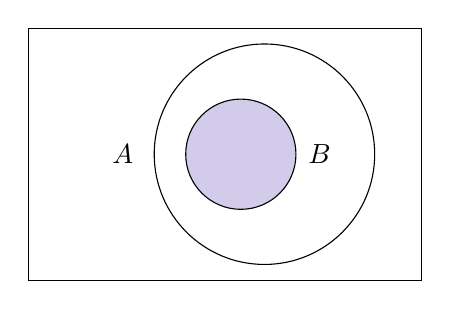
\begin{tikzpicture}
                \path[draw]
                    (0,0) -- (5,0) -- (5,3.2) -- (0,3.2) -- cycle; 
                \draw
                    (3,1.6) circle[radius=1.4];
                \filldraw[color=black,fill=Periwinkle!30]
                    (2.7,1.6) circle[radius=0.7]; 
                \node 
                    at (1.2,1.6) {\(A\)}; 
                \node 
                    at (3.7,1.6) {\(B\)}; 
            \end{tikzpicture}
            \caption{Venn diagram showing \(P(A\cap{}B) = P(B)\), with the indicated probability highlighted.}
        \end{figure}
        \item \(P(A\cup{}B) = P(B)\).\begin{figure}[h]
            \centering
            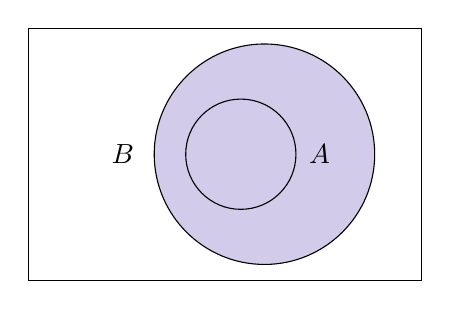
\begin{tikzpicture}
                \path[draw]
                    (0,0) -- (5,0) -- (5,3.2) -- (0,3.2) -- cycle; 
                \filldraw[color=black,fill=Periwinkle!30]
                    (3,1.6) circle[radius=1.4];
                \draw
                    (2.7,1.6) circle[radius=0.7]; 
                \node 
                    at (1.2,1.6) {\(B\)}; 
                \node 
                    at (3.7,1.6) {\(A\)}; 
            \end{tikzpicture}
            \caption{Venn diagram showing \(P(A\cup{}B) = P(B)\), with the indicated probability highlighted.}
        \end{figure}
    \end{enumerate}
    \item In the game of ``odd man out'' each player tosses a fair coin. If all the coins turn up the same except for one, the player tossing the different coin is declared the
    odd man out and is eliminated from the contest. Suppose that three people are playing. What is the probability that someone will be eliminated on the first toss?\begin{solution}
        Since there are only three people playing, the only way for someone to not be eliminated is if all their coins are the same. If we let \(A\) be the event that someone is 
        eliminated on the first toss, then \(A^C\) is the event that no one is, and \(P(A)\) will be given by \(1 - P (A^C)\). Out of all the possible outcomes 
        of the coin flips (of which there are 8: \(\lbrace{}\)HHH, TTT, HTT, HHT, HTH, THH, TTH, THT\(\rbrace{}\)),
        two of them have all three coins showing up as the same face. Thus, \(P(A^C) = \frac{1}{4}\), so the probability that someone is eliminated
        on the first round is \(\frac{3}{4}\), or 0.75. 
    \end{solution}
    \begin{minipage}[t]{.14\textwidth}
        \vspace{0pt}
        
\includegraphics[width=2cm]{nerd_maddy.png} 
    \end{minipage}%
    \fbox{
    \begin{minipage}[t]{.76\textwidth}
        \vspace{0pt}
        \textbf{Nerd Interjection!} You'll notice that the previous problem essentially boiled down to a counting problem. If you're familiar with combinatorics, you might remember there's 
        a handy way of counting ways to do something that involve successes and failures: the \textbf{binomial coefficients}. We'll see later that there's a way of formalizing a 
        theorem for similar situations, which should give us solutions like this next one.
    \end{minipage}%
    }\begin{solution}
        The probability that the result of one player's coin toss is different from the other two's is described by the binomial distribution. We have 0.5 for the probability of either 
        heads or tails, three trials (because there are three players), and we wish to find one ``success'' (i.e.\ that player's result is different). Thus,\[
            \binom{3}{1} {(1-0.5)}^{3-1} 0.5^{1} = 3 \cdot 0.25 \cdot 0.5 = 0.375~\text{or}~\frac{3}{8}.   
        \] But wait! This isn't our answer from earlier. Well, that's because we need to multiply it by 2. ``Success'' here can mean either heads or tails, depending on what
        the other two flipped, but we've only calculated for one of the cases (let's say heads). Thus, without loss of generality\footnote{These four words are \textit{very} important in combinatorics. 
        Look it up if you're interested! I'm not great at explaining it.}, 
        we say that the case in which the player eliminated flips tails is the same as the case where they flip heads, and we multiply this result by 2, giving us \(\frac{3}{4}\) or 0.75. 
    \end{solution}
    We can actually also solve item \#{}5 with the binomial distribution, but we'll save that for when we actually learn the binomial distribution because it's a bit more involved than 
    this one is. But if you're curious, here are the funny numbers:\[
        \binom{3}{1} {\biggl(\frac{1}{6}\biggr)}^1 {\biggl(\frac{5}{6}\biggr)}^{3-1} +  \binom{3}{2} {\biggl(\frac{1}{6}\biggr)}^2 {\biggl(\frac{5}{6}\biggr)}^{3-2} + \binom{3}{3} {\biggl(\frac{1}{6}\biggr)}^3 
        {\biggl(\frac{5}{6}\biggr)}^{3-3} = \frac{91}{216},
    \] which is exactly the answer we got earlier (that I was too lazy to simplify). 
    \item An urn contains twenty-four chips, numbered 1 through 24. One is drawn at random. Let \(A\) be the event that the number is divisible by 2 and let \(B\) be the event
    that the number is divisible by 3. Find \(P(A\cup{}B)\).\begin{solution}
        There are 12 numbers divisible by 2 within the range of \([1,24]\), which means the probability of drawing one is \(\frac{12}{24} = \frac{1}{2} \). Likewise, there are 
        8 numbers divisible by 3 within the range, which gives the probability of \(\frac{8}{24} = \frac{1}{3}\). We know that \(P(A\cup{}B) = P(A) + P(B) - P(A\cap{}B)\), 
        which means we just need to solve for the intersection of these two events. We know that if a number is divisible by both 2 and 3, then it is divisible by 6. Thus, \(P(A\cap{}B)\)
        is equivalent to \(P(\text{the number drawn is divisible by 6})\). There are 4 such numbers in the given range, which gives \(\frac{4}{24} = \frac{1}{6}\) for our probability. 
        Finally, substituting these values gives us \(
            \frac{1}{2} + \frac{1}{3} - \frac{1}{6} = \frac{2}{3}
        \) for the probability that a number is divisible by 2 or 3. 
    \end{solution}
    \item If State's football team has a 10\% chance of winning Saturday's game, a 30\% chance of winning two weeks from now, and a 65\% chance of losing both games, what
    are their chances of winning exactly once?\begin{solution}
        Let \(A\) be the event that they win Saturday's game and \(B\) be the event that they win two weeks from now. Then, \(P(A) = 0.1\), \(P(B) = 0.3\), and \(P(A^C\cap{}B^C) = 0.65\).
        We need to find the probability that they win one but not the other, which, as we've shown repeatedly thus far, is \(P(A\cup{}B) - P(A\cap{}B)\). We know by DeMorgan's laws that 
        \({(A\cup{}B)}^C = A^C\cap{}B^C\), so \(1-P(A^C\cap{}B^C) = 1-0.65 = 0.35 = P(A\cup{}B)\). Now, we just need to find \(P(A\cap{}B)\), which thankfully we have a formula for, given 
        \(P(A)\), \(P(B)\), and \(P(A\cup{}B)\). Therefore,\[
            P(A\cup{}B) - P(A\cap{}B) = 0.35 - (0.1 + 0.3 - 0.35) = 0.35 - 0.5 = 0.3 
        \] is the probability that the team will win exactly once. 
    \end{solution}
    \item Events \(A_1\) and \(A_2\) are such that \(A_1 \cup{} A_2 = S\) and \(A_1 \cap A_2 = \emptyset\). Find \(p_2\) if \(P(A_1) = p_1\), \(P(A_2) = p_2\), and
    \(3p_1 - p_2 = \frac{1}{2}\).\begin{solution}
        \(A_1 \cup{} A_2 = S\) and \(A_1 \cap A_2 = \emptyset\) tell us that \(p_1\) and \(p_2\) are mutually exclusive, and that \(P(A_1\cup{}A_2) = P(S) = 1\). Thus, \(p_1 + p_2 = 1\). 
        We can rewrite this equation as \(p_1 = 1 - p_2\) and substitute it into the given equation. Then,\[
            3(1-p_2) - p_2 = \frac{1}{2} \Longleftrightarrow
            3 - 4p_2 = \frac{1}{2} \Longleftrightarrow
            -4p_2 = -\frac{5}{2} \Longleftrightarrow
            p_2 = \frac{5}{8},
        \] which gives us our value for \(p_2\). 
    \end{solution}
    \item Consolidated Industries has come under considerable pressure to eliminate its seemingly discriminatory hiring practices. Company officials have agreed that during
    the next five years, 60\% of their new employees will be women and 30\% will be members of racial minorities. One out of four new employees, though, will be a white man. What percentage
    of their new hires will be minority women?\footnote{I changed the phrasing of this question because it goes against my morals to use the word ``females''.}\begin{solution}
        Consider randomly selecting an employee out of Consolidated Industries' new hires. Let \(A\) be the event that the employee is a woman, \(B\) be the event that the 
        employee is a member of a minority group, and \(C\) be the event that the employee is a white man. The probabilites for all these events are already given, with \(C\)
        obviously being exclusive from the other two. We are tasked to find \(P(A\cap{}B)\), which we know will be equal to \(P(A) + P(B) - P(A\cup{}B)\). We know all of 
        these except the last term, so we will have to figure it out.\par 
        If one out of every four employees will be a white man, then that means the remaining three will either be women or members of minority groups. Thus, \(P(A\cup{}B) = 0.75\). 
        Now that we have all our values, we can just substitute.\[
            P(A\cap{}B) = 0.6 + 0.3 - 0.75 = 0.15
        \]Thus, 15\% is the percentage of new hires that will be women from minority groups. 
        \end{solution}
        \begin{minipage}[t]{.14\textwidth}
            \vspace{0pt}
            
\includegraphics[width=2cm]{nerd_maddy.png} 
        \end{minipage}%
        \fbox{
        \begin{minipage}[t]{.76\textwidth}
            \vspace{0pt}
            \textbf{Nerd Interjection!} I thought it was very quaint that they included a situation like this in the  sample problems, 
            even if they did use the word ``females'' (shudders). People really need to recognize the biases, both 
            personal and systemic, against members of minority groups. Especially those who try to gaslight everyone into thinking there isn't a problem!\par What, you thought I 
            could only talk about math in these? 
        \end{minipage}%
        }
    \item Three events---\(A\), \(B\), and \(C\)---are defined on a sample space, \(S\). Given that \(P(A) = 0.2\), \(P(B) = 0.1\), and
    \(P(C) = 0.3\), what is the smallest possible value for \(P\big({(A\cup B \cup C)}^C\big)\)?\begin{solution}
        Asking what the smallest possible value for \(P\big({(A\cup B \cup C)}^C\big)\) is is equivalent to asking what the \textit{largest} possible value for \(P(A\cup{}B\cup{}C)\)    
        is, as any increase to the value of this probability will simultaneously decrease \(P\big({(A\cup B \cup C)}^C\big)\). Then, the largest probability for the union of these three 
        events is when all three of them are mutually exclusive from each other, and when we can thus add them all together to find \(P(A\cup{}B\cup{}C)\). This value is 0.6, and 
        subtracting it from 1 gives us 0.4 as the smallest possible value for \(P\big({(A\cup B \cup C)}^C\big)\). 
        \end{solution}
    \item A coin is to be tossed four times. Define events \(X\) and \(Y\) such that\[ 
        X\!:~\text{first and last coins have opposite faces},~Y\!:~\text{exactly two heads appear}
    \] Assume that each of the sixteen head/tail sequences has the same probability. Evaluate\begin{enumerate}
        \item \(P(X^C\cap{}Y)\)\begin{solution}
            This probability is asking for the cases in which the first and last coins have the same faces, and exactly two heads appear. From inspection, we notice that this only happens 
            when the sequence of tosses is \(THHT\) or \(HTTH\). Thus, dividing this by the total number of possible outcomes (16, I won't bother listing them but it's just \(2^4\) because
            2 outcomes, 4 coins) gives us \(\frac{2}{16} = \frac{1}{8} = 0.125\). 
        \end{solution}
        \item \(P(X\cap{}Y^C)\)\begin{solution}
            This probability is asking for the cases in which the first and last coins are opposite, and there aren't exactly two heads. From inspection, we notice that there will never be four or zero 
            heads, because the first and last faces have to be different. Then, the valid sequences are \(HTTT\), \(HHHT\), \(THHH\), and \(TTTH\). Thus, the probability of one of these 
            occuring is simply \(\frac{4}{16} = \frac{1}{4} = 0.25\).
        \end{solution}
    \end{enumerate} 
    \item Two dice are tossed. Assume that each possible outcome has a \(\frac{1}{36}\) probability. Let \(A\) be the event that the sum of the faces showing is 6, and let \(B\) be the event that
    the face showing on one die is twice the face showing on the other. Calculate \(P(A \cap{} B^C)\).\begin{solution}
        To be honest, I think this question is rather vague, particularly the ``Assume that each possible outcome has a \(\frac{1}{36}\) probability''. I'm taking it to mean that each outcome of both
        dice rolled together has a probability of \(\frac{1}{36}\), and not that the dice individually have 36 possible sides, because if that were the case then maybe they would've just said that.
        Also it works out nicely that there are 36 possible outcomes for two six-sided dice. Just very confusing why they chose to word it this way.\par 
        If we analyze \(A\cap{}B\), we identify two cases: \((2,4), (4,2)\). If we exclude these but still consider the outcomes with a sum of 6, we have \(\lbrace (1,5), (5,1), (3,3) 
        \rbrace\), for a total of three possible outcomes wherein the sum is 6, but the face on one die is not twice the face on the other. Therefore, the probability of \(A\cap{}B^C\) is \(\frac{3}{36} 
        = \frac{1}{12}\). 
    \end{solution}
    \item Let \(A\), \(B\), and \(C\) be three events defined on a sample space, \(S\). Arrange the probabilities of the following events from smallest to largest:
    (a) \(A\cup B\); (b) \(A \cap B\); (c) \(A\); (d) \(S\); (e) \((A \cap{} B) \cup (A \cap C) \).\begin{solution}
        We know that given two events \(A\) and \(B\), \(A\cap{}B \leq A,B \leq A\cup{}B\), and that \(S\) is always equal to 1, so we just need to figure out where to put in \((A\cap{}B)\cup(A\cap{}C)\). 
        Well, from set theory (which you should know), we know that \((A\cap{}B)\cup(A\cap{}C) = A\cap{}(B\cup{}C)\), so we can see it's really just another intersection of \(A\), but with a set that is 
        larger than \(B\), so we put it in between \(A\cap{}B\) and \(A\).\par Therefore, our final ordering is \(A\cap{}B\leq(A\cap{}B)\cup(A\cap{}C)\leq{}A\leq{}A\cup{}B\leq{}S\).\footnote{You'll notice 
        I used less than or equal to instead of strictly less than. Technically speaking, any of these events could be equal to the next one, because the question didn't go the tiny extra step of saying 
        \(A\neq{}B\neq{}C\), but that's just me being picky about semantics. We got it anyway. } 
    \end{solution}
    \item Lucy is currently running two dot-com scams out of a bogus chatroom. She estimates that the chances of the first one leading to her arrest are one in ten; the ``risk''
    associated with the second is more on the order of one in thirty. She considers the likelihood that she gets busted for both to be 0.0025. What are Lucy's chances of avoiding
    incarceration?\begin{solution}
        Let \(A\) be the event that she gets caught for the first scam, and \(B\) be the event that she gets caught for the second. We are looking for the probability that she doesn't get caught for either, 
        or symbolically, \(P\big({(A\cup{}B)}^C\big)\). Since we have the probabilites for both events and their intersection. We can just do simple substitution.\[
            P\big({(A\cup{}B)}^C\big) = 1 - P(A\cup{}B) = 1 - \biggl(\frac{1}{10} + \frac{1}{30} - \frac{25}{10000}\biggr) = 1 - \frac{157}{1200} = \frac{1043}{1200} \approx 0.8691666\ldots
        \] Therefore, Lucy has a \(\frac{1043}{1200}\) or roughly 87\% chance of evading capture. Go Lucy!
    \end{solution}
\end{enumerate}

\pagebreak
\section*{2.4: Conditional Probability}
\textit{This section has 54 exercises, so it's probably unreasonable for me to finish them all, but I'll see how far I can get before getting bored. }
\begin{enumerate}
    \item Suppose that two fair dice are tossed. What is the probability that the sum equals 10 given that it exceeds 8?\begin{solution}
        Let the probability that the result is 10 be \(A\). \(P(A) = \frac{3}{36}\), because there are three combinations that give 10, namely \(\lbrace(4,6),(5,5),(6,4)\rbrace\). Meanwhile, let the probability 
        that the sum  exceeds 8 be \(B\). \(P(B) = \frac{10}{36}\), because there are ten combinations that result in a sum above 8 (which I won't list anymore). Since 10 is always greater than 8, 
        \(P(A\cap{}B) = P(A)\). Thus, substituting, we have\[
            P(A|B) = P(A) / P(B) = \frac{3}{36} \cdot \frac{36}{10} = \frac{3}{10},
        \] for the probability that the sum of the dice is 10 given that it is greater than 8. 
    \end{solution}
    \item Find \(P(A\cap{}B)\) if \(P(A) = 0.2\), \(P(B) = 0.4\), and \(P(A|B) + P(B|A) =0.75\).\begin{solution}
        We can solve for this by simply substituting the first two equations into the last one.\[
            \frac{P(A\cap{}B)}{0.4} + \frac{P(B\cap{}A)}{0.2} =0.75 \Longleftrightarrow P(A\cap{}B) \big(7.5\big) = 0.75 \Longleftrightarrow P(A\cap{}B) = 0.1. 
        \] Simplification of fractions has been omitted for space. 
    \end{solution}
    \item If \(P(A|B) < P(A)\), show that \(P(B|A) < P(B)\).\begin{proof}
        Finally, some proving so I can feel alive again. Here, we just do straightforward algebra. By the given,\[
            \frac{P(A\cap{}B)}{P(B)} < P(A) \Longleftrightarrow
            P(A\cap{}B) < P(A)\,P(B)
        \] Now, if we try to solve for \(P(B|A)\), we get\[
            P(B|A) = \frac{P(B\cap{}A)}{P(A)} = \frac{P(A\cap{}B)}{P(A)}< \frac{P(A)\,P(B)}{P(A)} = P(B),
        \] which proves the statement. 
    \end{proof}
\end{enumerate}

\end{document}